\documentclass[a4paper,12pt]{article}
\usepackage{amssymb}
\usepackage{geometry}
\usepackage{graphicx}
\usepackage{colortbl}
\usepackage{wrapfig}
\geometry{margin=1in}



\begin{document}

Dustin Kane

CMSI 370-01

November 24, 2015

\begin{center}
\section*{Assignment 1124: Dream Design}
\subsection*{The Ultimate Heads-Up Display with Microsoft HoloLens}
\end{center}

\section{Introduction}
\subsection{A Bicycle For Our Minds}

Steve Jobs, the cofounder of Apple Computers, liked to tell a story. He found a study that measured the distance versus energy consumption for various animals. The study found the condor to be the most efficient animal and put humans fairly far down the list. However, Scientific American decided to test the efficiency of a human on a bicycle. A person on a bicycle was by \emph{far} the most efficient animal on the planet. With that in mind, Steve Jobs said this:

\begin{quote} 
    ``And that's what a computer is to me. What a computer is to me is it's the most remarkable tool that we've ever come up with, and it's the equivalent of a bicycle for our minds.'' - Steve Jobs [1]
\end{quote}

Computers are bicycles for our minds. They are augmentations to our intellect. Or, at least they should be. Computers today do not really achieve this vision. The Scientific American test implied that the bicycle was the extension of a person; a person \emph{on} a bicycle \emph{is} the most efficient animal. A modern computer is not an extension of a person. It is a tool: an interface that a person has to interact with. A computer is more like a parking meter or a cashier at a store; it isn't an extension of the person using it by any stretch of the imagination. Smart phones feel more like an extension of a person; people are tethered to their phones and sometimes filter every thought and action through it. But the way they interface with it is still like the way they interact with a garage-door opener or a television remote. Computers are incredibly useful, but their interfaces are essentially just consoles: a set of buttons and switches that make the machine do something. To create an interface that lives up to the dream of the Bicycle of the Mind, we need an interface that we feel connected to and integrated with.

\subsection{Realizing the Mind-Bicycle Dream}
To put it in more concrete terms, a bicycle takes the existing human behavior of movement and improves it by making it faster and more efficient. A computer should take existing human mental behavior and improve it by making it faster, more efficient, and even more. Instead of giving you turn-by-turn directions through Google Maps, the computer should improve your ability to \emph{know} where to go. Instead of allowing a user to look up an actress on IMBD, a computer should improve the ability of the user to \emph{remember} what movies she was in. Instead of providing the user with a calculator, the computer should improve the ability of the user to \emph{calculate} arithmetic problems. I'm not suggesting the computer augment the brain to be more effective; that would be like suggesting a bicycle allows a man to move his legs faster. The problem is the way we interact with computers is more akin to the way we interact with a servant or a secretary: we ask it questions and we give it commands. We do not interact with a bicycle by telling it to go faster: we interact with a bicycle by moving our legs in a way that is fairly similar to the way we would move them without the bicycle, and the bicycle augments that behavior. In the same way, we should interact with a computer by, essentially, doing what we do without a computer and the computer handles the rest.

I imagine a computer that, instead of a screen, superimposes information on our field of vision through a pair of glasses. The computer sees what we see and hears what we hear. We give the computer instructions by, essentially, thinking out loud. Just like we slightly alter the motion of running to apply it to a bicycle, we slightly alter our way of thinking to apply it to this interface. I believe this kind of interface could be created today using the existing concept of a ``Heads-Up Display'' [2] and implementing it with the Microsoft HoloLens hardware [4].

\section{The Heads-Up Display}

\subsection{Heads-Up Displays in Military Aircraft}

\begin{wrapfigure}{r}{0.5\textwidth}
\centering
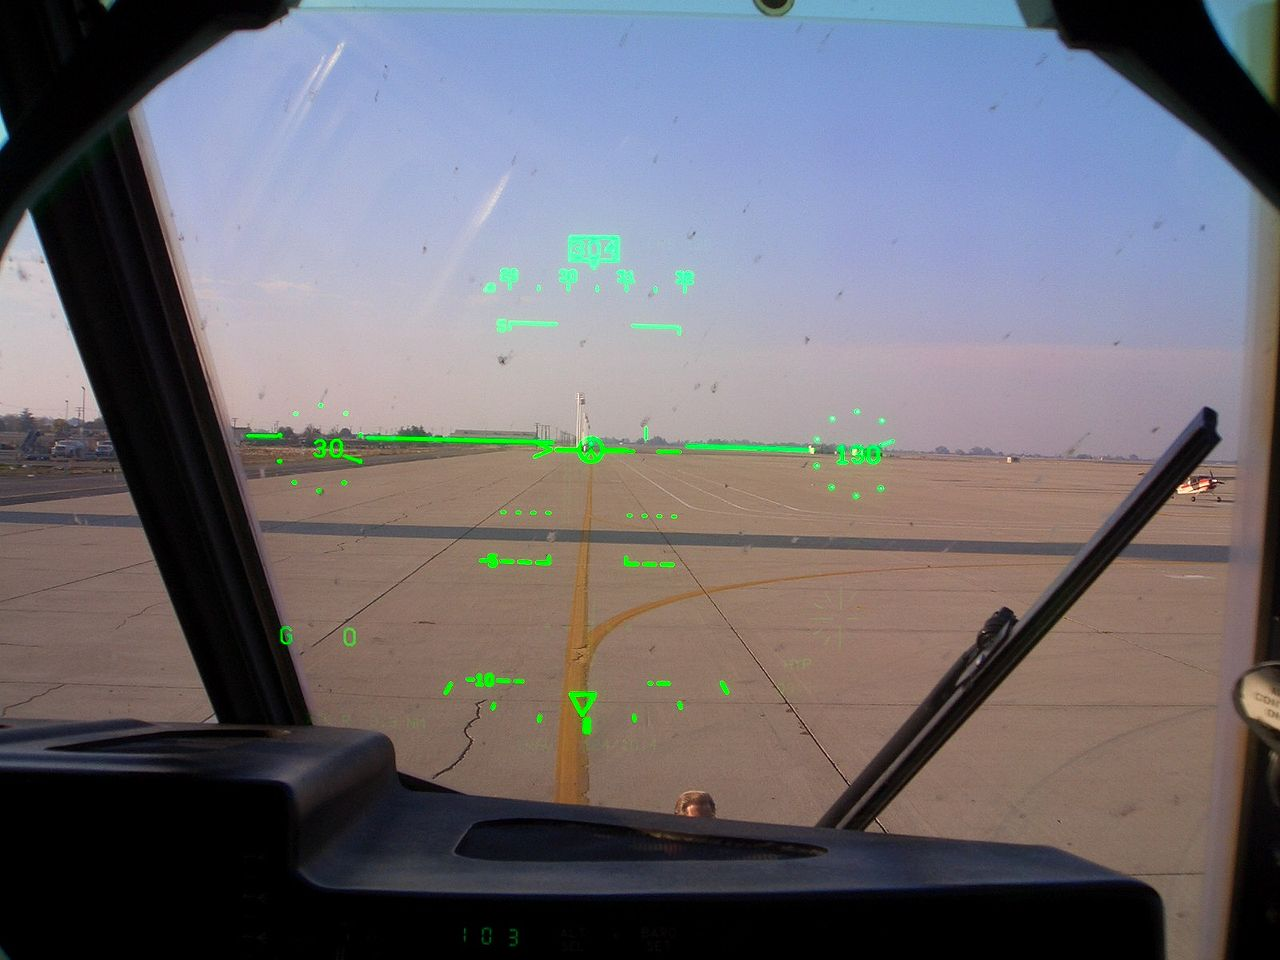
\includegraphics[width=0.5\textwidth]{jethud}
\caption{HUD of a C-130J [3]}
\end{wrapfigure}

A Heads-Up Display is a kind of instrument that super-imposes information over what the user would otherwise be looking at. This kind of instrument is mostly used in military aircraft. The fighter jet has a transparent screen in the cockpit between the pilot and the front windshield. The pilot can now look at readings from his instruments while looking straight ahead; he doesn't have to look down at his instruments, he keeps his head up, hence the name Heads-Up Display.

This interface does more than save the pilot from having to move his head. Like the bicycle, the jet is meant to be an extension of the human being. The pilot looks straight forward at where he's flying. With the Heads-Up display, instead of interacting with his instruments in a kind of transactional way---looking down at them, querying them for information---the pilot has the relevant information right in front of him. The action of the pilot is the same as if the instruments weren't there, yet he still gets the benefit of having the information from them. His ability to fly is augmented by the availability of the information from the Heads-Up Display.

\subsection{A Heads-Up Display For Everyday Life}

The dream interface takes the Heads-Up Display out of the fighter jet and into the hands of the average person. Instead of displaying altitude and air speed, the Heads-Up Display can display turn-by-turn directions, restaurant reviews, news articles, and more. Instead of looking down at a phone for directions, or listening to a voice say to ``use the second lane to turn right onto the Christopher Columbus Transcontinental Freeway I-10,'' the user can look, straight ahead, at where they are going with an arrow showing them exactly what lane to drive in and what direction to go in. Here, the interface allows the user to behave as if they already knew where they were going. Then, a breaking news banner could scroll across their view telling them there has been a terrible accident somewhere. Here, the interface allows the user to behave as if they were really well informed; they didn't actively seek out the news, they act as if they already knew it.

\subsection{Augmented Reality}


Similar types of interfaces already exist, and they go by the name \emph{augmented reality}. 
\begin{wrapfigure}{l}{0.5\textwidth}
\centering
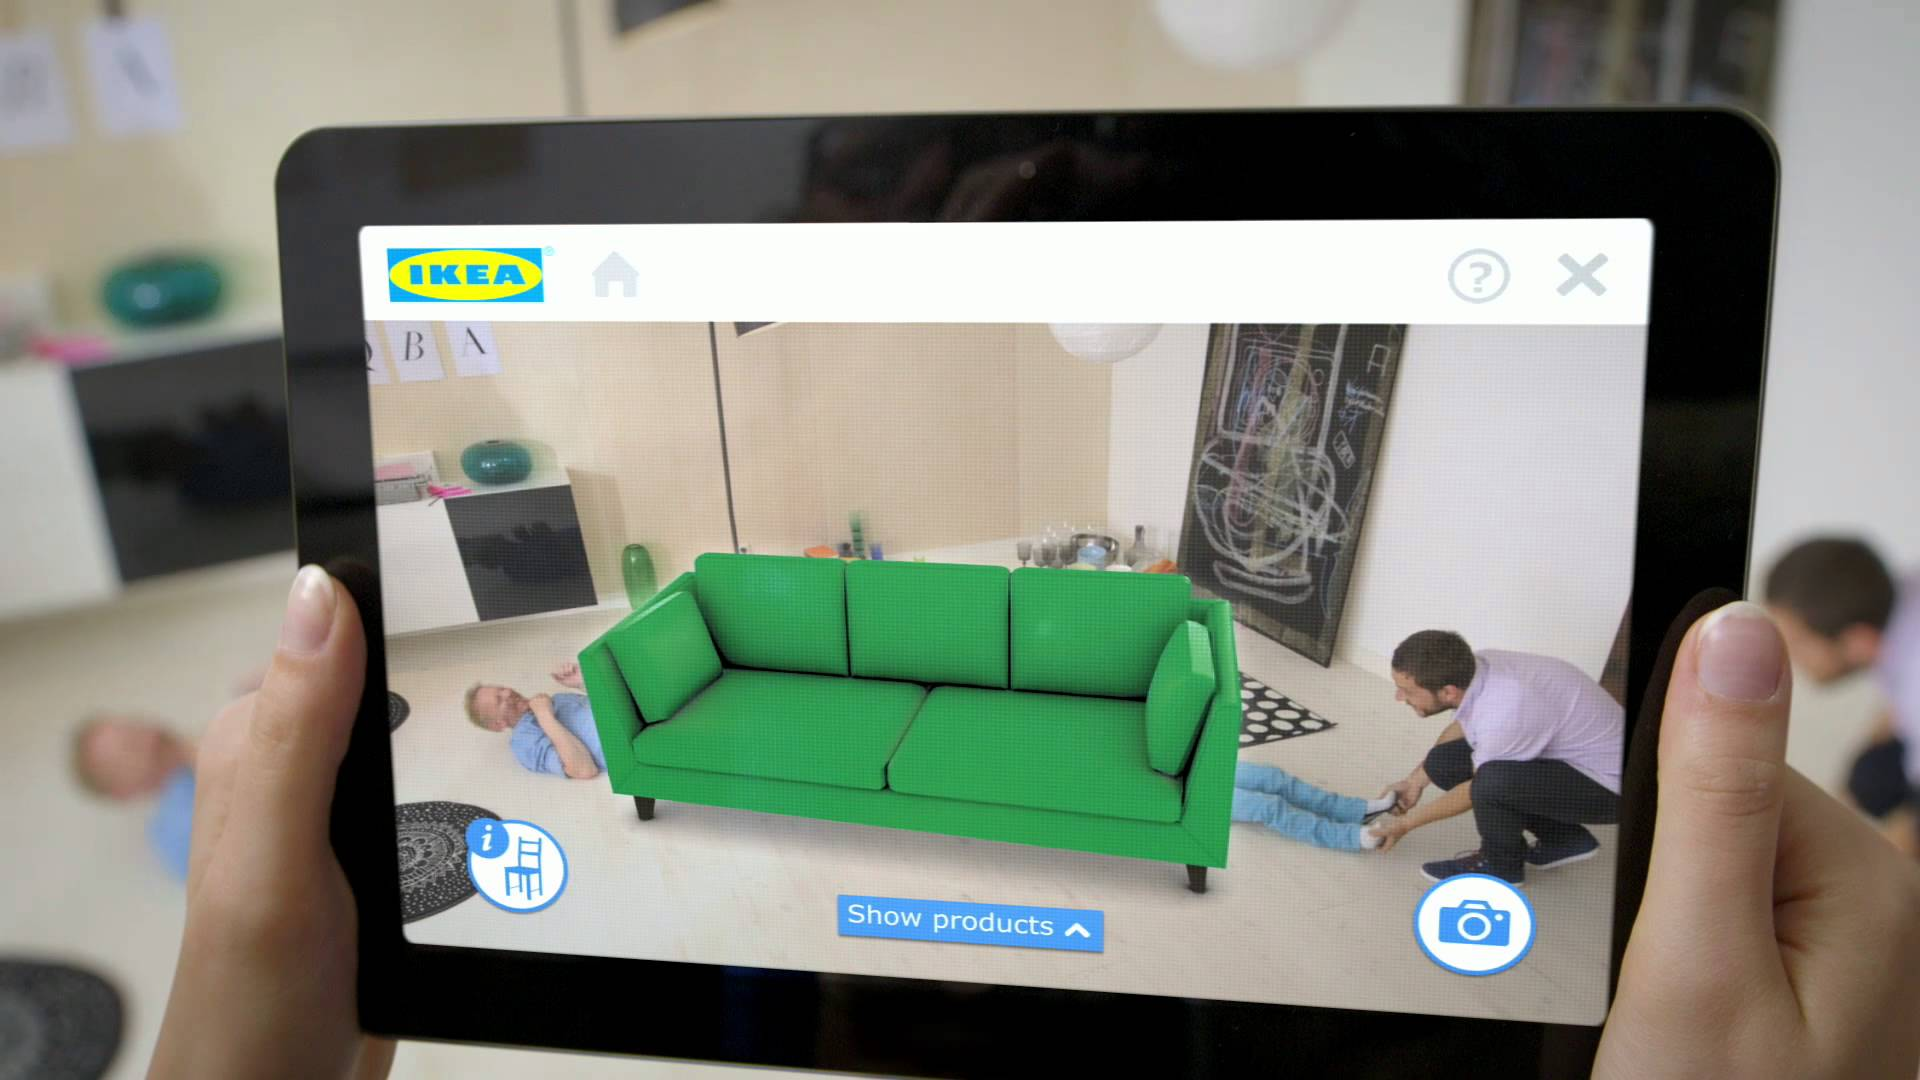
\includegraphics[width=0.5\textwidth]{ikea}
\caption{IKEA Catalog app [5]}
\end{wrapfigure}


Augmented reality refers to computers ``augmenting'' the real, physical world [4]. Figure 2 shows the IKEA Catalog app [5]. This app allows you to use your mobile device's camera to see what a room would look like with IKEA furniture. The app overlays the computer-generated furniture onto the image from the camera. The furniture is manipulable using the touch screen of the device. This is a favorable interface because it enhances something the user already does without a computer: visualizing how furniture will look in a room. This is something a user would, otherwise, do with their imagination. Technology comes in and creates the actual image to create a more accurate depiction of what the furniture will actually look like.

\begin{wrapfigure}{r}{0.5\textwidth}
\centering
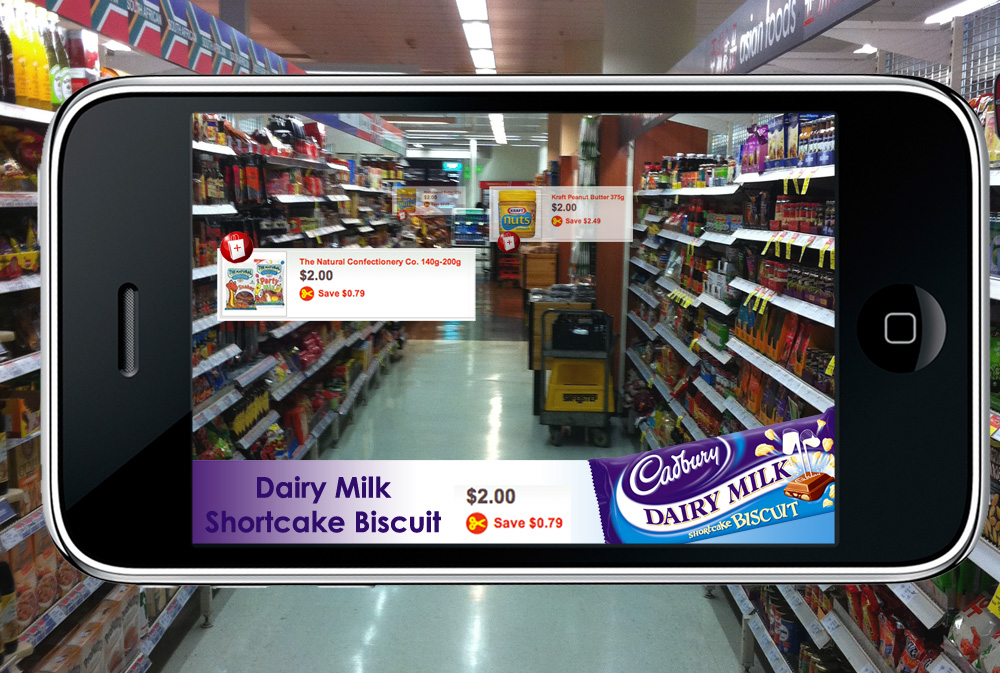
\includegraphics[width=0.5\textwidth]{coupons}
\caption{This app displays coupons and alternative pricing for items at a grocery store [6]}
\end{wrapfigure}

Figure 3 provides another example. This app shows the user coupons and alternate prices for items at a grocery store. The user points their phone's camera at items at the store and the app overlays prices and coupons next to the items in the image. This is a better interface than searching for prices online because it enhances the user's knowledge of prices. Instead of asking a third party, the user is presented the information next to the items in their view. The user behaves as if they knew the prices already, but they are actually being supplied with the beneficial information by the computer.



Matthew Buckland wrote an interesting essay on the potential applications of augmented reality to social networking [7]. Illustrated in Figure 4, Buckland imagines an interface where the user can hold up their phone's camera to a row of houses and get various data from social media. The data may include information about an upcoming block party, or a location on a map. It could also have tags next to each house representing profiles of each resident with quick buttons to get in contact with each of these people. Here, the computer is enhancing the user's ability to recognize houses and the people who live in them. It's also incredibly efficient because it includes interactive buttons for things like messaging right next to the houses in the image. This example is the most similar to the interface I'm proposing.

\begin{figure}
\centering
\includegraphics[width=\textwidth]{social}
\caption{A concept design of an augmented reality app centered around social media [7]}
\end{figure}

There is a problem with each of these examples, however. In Figures 2-4, there is a visible device. For this interface to reach its full potential, there cannot be a visible device. First, the edges of the device obstruct the user's view; in Figure 3 we cannot see what items are behind the black bars of the iPhone. Second, the entire field of view is not augmented by the interface; users have to look at the world through their device, either holding it uncomfortably close to their face or getting a very small porthole to see the augmented world. Finally, the user's hands aren't free. The user must hold the device up, making them unable to use their hands in ways they normally would. This interface would be impossible to use for getting directions while driving, or instructions while cooking, for example. For this interface to realize its potential it must include the user's entire view, it must not obstruct any part of the user's view, and it must be hands free. 



\section{The Microsoft HoloLens}

\subsection{The Augmented Reality Device}

In January 2015, Microsoft unveiled the HoloLens, a device designed for augmented reality [9]. The HoloLens is a headset that displays images on a transparent screen right in front of the user's eyes. Unlike many \emph{virtual reality} headsets released prior to it that create an \emph{entirely} virtual world, the HoloLens is transparent and lays computer-generated images over the user's view of the real world. As Microsoft puts it on their website: 

\begin{quote}
``Microsoft HoloLens generates a multi-dimensional image visible to a user so that he or she perceives holographic objects in the physical world. Holographic objects seen with Microsoft HoloLens can be placed in physical locations you choose, move according to their own rules, or remain in a specific location within your field of view regardless of where you are or in which direction you are looking.'' - Microsoft [10]
\end{quote}

\subsection{What Can It Do?}

The key feature of the HoloLens is that, through its sensors, and complex processor, it can react to user gestures. As Microsoft puts it: 

\begin{quote} 
    ``The holograms you'll see with Microsoft HoloLens can appear life-like, and can move, be shaped, and change according to interaction with you or the physical environment in which they are visible. Use gestures to create, shape, and size holograms. Use your gaze to navigate and explore. Use your voice to communicate with your apps. Microsoft HoloLens understands your movements, gaze, and voice, enabling you to interact with content and information naturally. Using holograms, you can place your digital content, such as apps, information, and even multi-dimensional videos, in the physical space around you, so you can interact with it.'' - Microsoft [10]
\end{quote}

The idea is the HoloLens can create virtual objects that can be manipulated by the user. It can sense the user's hands and recognize gestures to allow for things like moving and interacting with objects. It also immerses the user in computer-generated images, using their entire field of view. 

It is able to do this with dedicated hardware. Microsoft says

\begin{quote}
    ``The HPU is custom silicon that processes a large amount of data per second from the sensors. Microsoft HoloLens understands gestures and where you look, and maps the world around you, all in real time.'' - Microsoft [11]
\end{quote}

Though Microsoft has only released a limited amount of detailed information about the device and how it works, based on live demos of users playing various video games and interacting with 3D models (all viewable on the HoloLens product page [12]), we can assume the device is fairly robust in its computing capabilities for things like image projection and complex gesture recognition. 

\section{The Dream Design: An Interactive Heads-Up Display with Microsoft HoloLens}

\subsection{Putting It All Together}



\section{Sources}


\begin{enumerate}
    \item https://www.brainpickings.org/2011/12/21/steve-jobs-bicycle-for-the-mind-1990/
    \item https://en.wikipedia.org/wiki/Head-up\_display
    \item https://en.wikipedia.org/wiki/Head-up\_display\#/media/File:C-130J\_Co\_Pilot\%27

    s\_Head-up\_display.jpg
    \item https://en.wikipedia.org/wiki/Augmented\_reality
    \item https://www.youtube.com/watch?v=vDNzTasuYEw
    \item http://augmentedpixels.com/wp-content/uploads/2013/11/augmented-reality-

    marketing.jpg
    \item http://matthewbuckland.com/?p=1041
    \item http://www.matthewbuckland.com/wp-images/futureofsocialnetworking02.png
    \item http://www.theverge.com/2015/1/21/7867593/microsoft-announces-windows-

    holographic
	\item https://www.microsoft.com/microsoft-hololens/en-us/faq
	\item https://www.microsoft.com/microsoft-hololens/en-us/hardware
    \item http://www.microsoft.com/microsoft-hololens/en-us
\end{enumerate}


\end{document}